%!TEX TX-program = xelatex
\documentclass[8pt]{article}

\usepackage{ctex}
\usepackage{graphicx}
\usepackage{enumitem}
\usepackage{geometry}
\usepackage{amsmath}
\usepackage{amssymb}
\usepackage{amsfonts}
\usepackage{tikz}
\usepackage{extarrows}
\usetikzlibrary{positioning}
\usetikzlibrary{svg.path}
\usepackage{xcolor}
\usepackage{soul}

\graphicspath{ {./images/} }

\author{高一(6)班\ 邵亦成\ 26号}
\title{10 奇偶性、单调性(难题)}
\date{2021年11月24日}

\geometry{a4paper, scale=0.8}

\begin{document}

	\maketitle

	\begin{enumerate}[label=\arabic*.]
		\item 已知实数$a\neq b$, 记函数$y=f(x)=|2x+a|-|2x+b|$. 若函数$y=|f(x+2)|$为偶函数, 则代数式$ab+a+2b$的最大值为?.
			~\\

			$$g(x)\xlongequal{\mathrm{def}}|f(x+2)|,$$

			$$f(x)\xlongrightarrow{\text{向左平移$2$单位}} \xlongrightarrow{\text{将$x$轴下方的部分翻折至$x$轴上方}}g(x).$$

			$$
			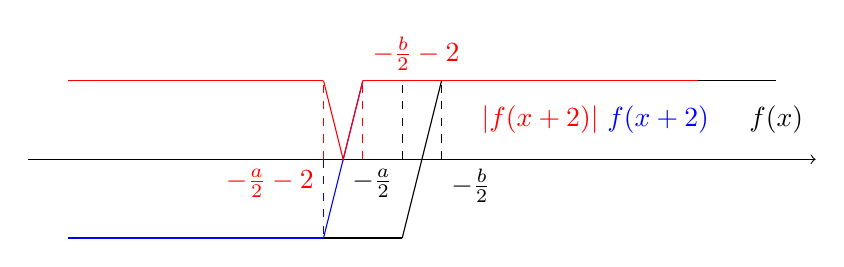
\begin{tikzpicture}[scale=0.5, declare function={f(\x) = abs(2*\x+1)-abs(2*\x-1);}]
	    		\draw[black, ->] (-10,  0)--( 10,  0);
	    		\draw[black, domain=-7:-0.5] plot({\x}, {f(\x)});
	    		\draw[black, domain=-0.5:0.5] plot({\x}, {f(\x)});
	    		\draw[black, domain=0.5:9] plot({\x}, {f(\x)}) node at (9, 1){$f(x)$};
	    		\draw[blue, domain=-9:-2.5] plot({\x}, {f(\x+2)});
	    		\draw[blue, domain=-2.5:-1.5] plot({\x}, {f(\x+2)});
	    		\draw[blue, domain=-1.5:7] plot({\x}, {f(\x+2)}) node at (6, 1){$f(x+2)$};
	    		\draw[red, domain=-9:-2.5] plot({\x}, {abs(f(\x+2))});
	    		\draw[red, domain=-2.5:-1.5] plot({\x}, {abs(f(\x+2))});
	    		\draw[red, domain=-1.5:7] plot({\x}, {abs(f(\x+2))}) node at (3, 1){$|f(x+2)|$};
	    		\draw[black, dashed] (0.5, 0)--(0.5, 2) node at (0.5, 0)[anchor=north west]{$-\frac{b}{2}$};
	    		\draw[black, dashed] (-0.5, 0)--(-0.5, 2) node at (-0.5, 0)[anchor=north east]{$-\frac{a}{2}$};
	    		\draw[blue, dashed] (-2.5, 0)--(-2.5, -2);
	    		\draw[red, dashed] (-1.5, 0)--(-1.5, 2) node at (-1.5, 2)[anchor=south west]{$-\frac{b}{2}-2$};
	    		\draw[red, dashed] (-2.5, 0)--(-2.5, 2) node at (-2.5, 0)[anchor=north east]{$-\frac{a}{2}-2$};
			\end{tikzpicture}
			$$

			故有

			$$-\frac{a}{2}-2-\frac{b}{2}-2=0 \Rightarrow a+b=-8 \Rightarrow b=-a-8,$$

			\begin{align*}
				ab+a+2b &= a(-a-8)+a+2(-a-8)\\
				&= -a^2-8a+a-2a-16\\
				&= -a^2-9a-16\\
				&\leq \dfrac{17}{4},
			\end{align*}

			等号成立条件

			$$(a, b)=\left(-\frac{9}{2}, -\frac{7}{2}\right).$$

		\item 已知函数$f(x)=\left\{\begin{array}{rl}x^2-x+3, &x\leq 1,\\x+\dfrac{2}{x}, &x>1.\\\end{array}\right.$ 设$a\in\mathbb{R}$, 若关于$x$的不等式$f(x)\geq\left|\dfrac{x}{2}+a\right|$在$\mathbb{R}$上恒成立, 求$a$的取值范围.
			~\\

			考虑$x\leq 1, $有

			$$x^2-x+3\geq \left|\frac{x}{2}+a\right|,$$

			即

			$$-x^2+x-3\leq \frac{x}{2}+a\leq x^2-x+3,$$

			即

			$$-x^2+\frac{1}{2}x-3\leq a\leq x^2-\frac{3}{2}x+3.$$

			而

			$$\max_{x\leq 1}\left(-x^2+\frac{1}{2}x-3\right)=-\frac{47}{16},\\\min_{x\leq 1}\left(x^2-\frac{3}{2}x+3\right)=\frac{39}{16},$$

			得

			$$a\in\left[-\frac{47}{16}, \frac{39}{16}\right].$$

			考虑$x>1, $有

			$$x+\frac{2}{x}\geq \left|\frac{x}{2}+a\right|,$$

			即

			$$-x-\frac{2}{x}\leq \frac{x}{2}+a\leq x+\frac{2}{x},$$

			即

			$$-\frac{2}{x}-\frac{3x}{2}\leq a\leq \frac{x}{2}+\frac{2}{x},$$

			而

			$$\max_{x>1}\left(-\frac{2}{x}-\frac{3x}{2}\right)=-2\sqrt{3},\\\min_{x>1}\left(\frac{x}{2}+\frac{2}{x}\right)=2,$$

			得

			$$a\in\left[-2\sqrt{3}, 2\right].$$

			综上,

			$$a\in\left[-\frac{47}{16}, 2\right].$$

	\end{enumerate}

\end{document}